\documentclass[t, pdftex]{beamer}  
%Use Cockrell School Theme.  Optional department name.  Must %ecape, i.e. use 
%backslash, to preserve spaces.  The default is ``Cockrell School of Engineering''
\usetheme[]{Cockrell}                 
%\usetheme[dept=Aerospace\ Engineering\ and\ Engineering\ Mechanics]{cockrell}                 
%\usetheme[dept=Biomedical\ Engineering]{cockrell}                 
%\usetheme[dept=Chemical\ Engineering]{cockrell}                 
%\usetheme[dept=Civil,\ Architectural\ and\ Environmental\ Engineering]{cockrell}                 
%\usetheme[dept=Electrical\ and\ Computer\ Engineering]{cockrell}                 
%\usetheme[dept=Mechanical\ Engineering]{cockrell}                 
%\usetheme[dept=Materials\ Science\ and\ Engineering]{cockrell}                 
%\usetheme[dept=Petroleum\ and\ Geosystems\ Engineering]{cockrell}                 

% Add preamble packages here
%\usepackage{etex}
%\usepackage[bigfiles]{media9}
%\graphicspath{{./figs/}}
\usepackage{bussproofs}
\usepackage[export]{adjustbox}
\usepackage{xcolor}
\usepackage{soul}

%Enable cancelto in math
\usepackage{cancel}
\renewcommand{\CancelColor}{\color{utorange}}
\usepackage{bbold}
\usepackage{hyperref}
\usepackage{datetime}
\newdate{date}{22}{06}{2017}


%Add bibliography file location for citiation
% \bibliography{example.bib}


\title{Presenting finite posets \\(with monotone maps?)}
\subtitle{... using string diagrams}
\author{Sam Balco}
% \institute{Special Event}
\date{\displaydate{date}}

\newenvironment{bprooftree}
  {\leavevmode\hbox\bgroup}
  {\DisplayProof\egroup}

\setlength{\parskip}{0.3cm}%


\begin{document}

%Creates title frame from title, subtitle, author, institute, and date above
\titleframe

%Supports table of contents
\frame{\frametitle{Outline}\tableofcontents}

%Section commands will define what's shown in TOC
\section{What are string diagrams?}

%First frame
\begin{frame}
    \frametitle{What are string diagrams?}
    They are a bit like legos!
    \begin{center}
        
\includegraphics{figures/lego.pdf}
    \end{center}
\end{frame}

\begin{frame}
    \frametitle{What are string diagrams?}
    We can combine legos/string diagrams in two different ways:
    \begin{center}
        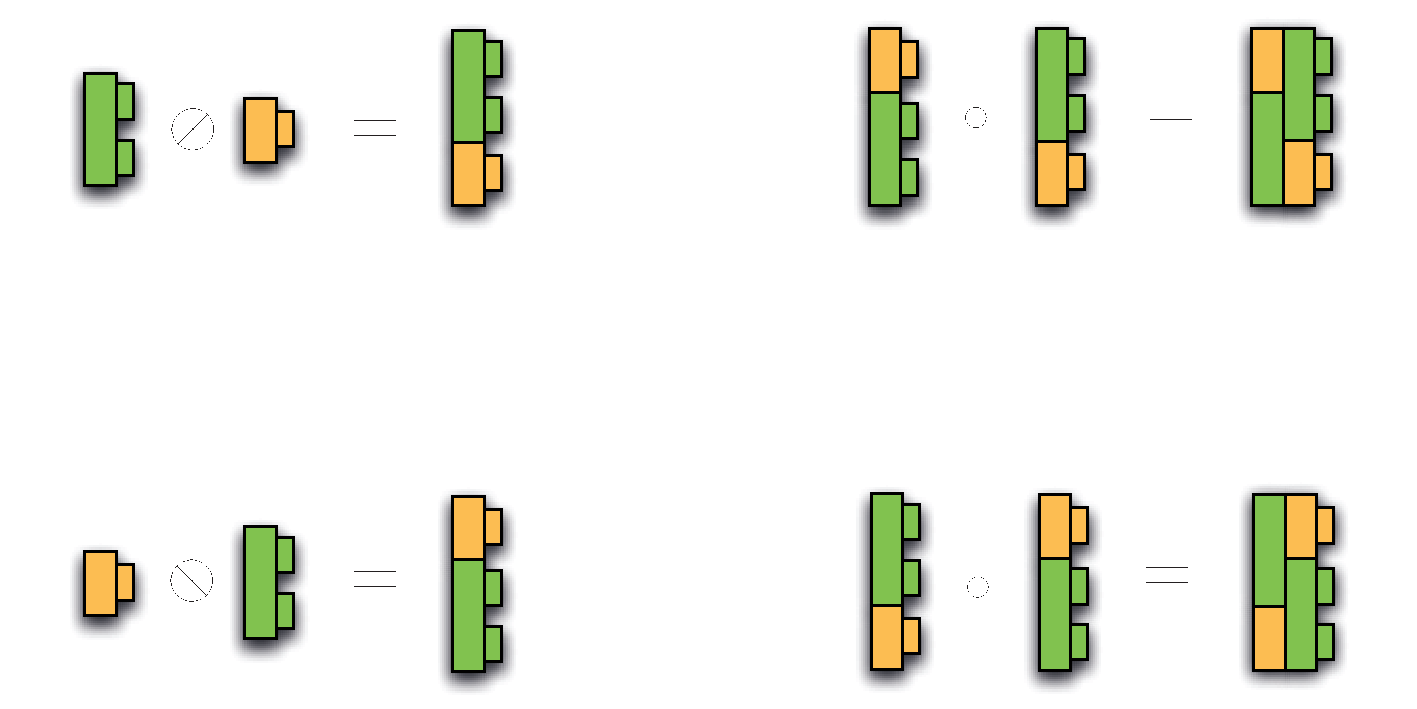
\includegraphics[width=\textwidth,keepaspectratio]{figures/lego2.pdf}
    \end{center}
\end{frame}

\begin{frame}
    \frametitle{What are string diagrams?}
    We can combine legos/string diagrams in two different ways:
    \begin{center}
        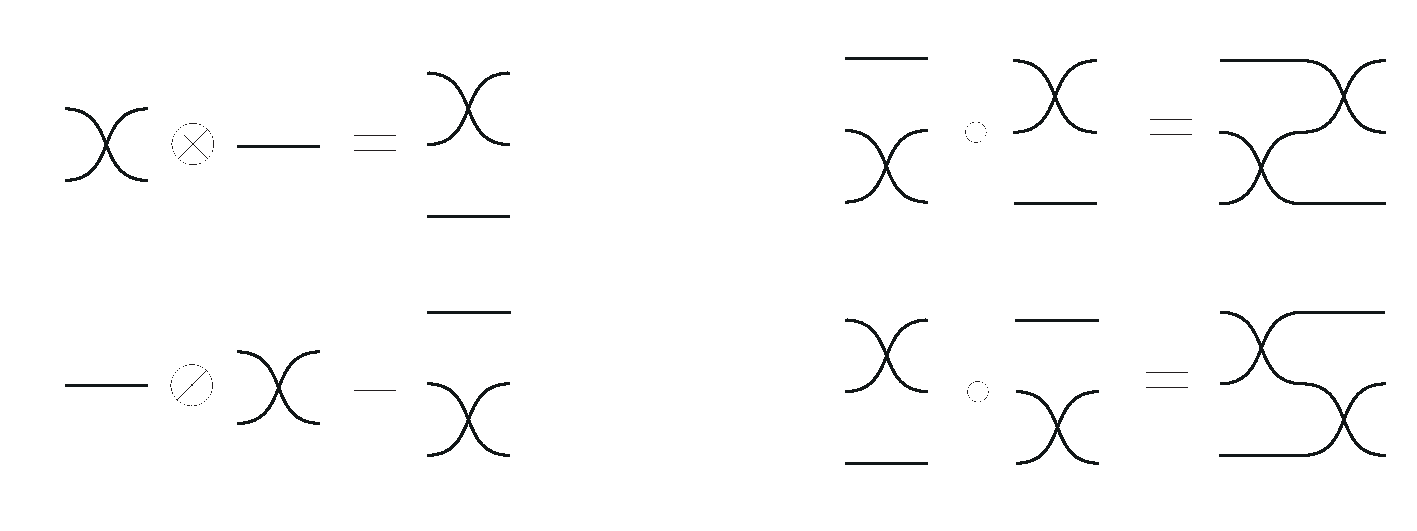
\includegraphics[width=\textwidth,keepaspectratio]{figures/lego3.pdf}
    \end{center}
\end{frame}

\section{String diagrams algebraically}

\begin{frame}
    \frametitle{String diagrams algebraically}
    We can assign each string a type, given by the number of input ports (on the left) and the number of output ports on the right:
    \begin{table}[]
        \centering
        \begin{tabular}{cccc}
            $id : 1 \to 1$ & 
            $\gamma : 2 \to 2$ & 
            $\mu \ : 2 \to 1$ & 
            $\eta \ : 0 \to 1$\\
            % \hrulefill & \hrulefill & \hrulefill & \hrulefill \\
            % & & & \\
            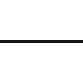
\includegraphics[valign=m, width=1cm]{figures/string2.pdf} & 
            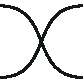
\includegraphics[valign=m, width=1cm]{figures/string1.pdf} & 
            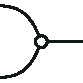
\includegraphics[valign=m, width=1cm]{figures/string4.pdf} &
            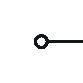
\includegraphics[valign=m, width=1cm]{figures/string3.pdf}
        \end{tabular}
    \end{table}
    \par
    % \begin{table}[]
    %     \centering
    %     \begin{tabular}{lll}
            
    %     \end{tabular}
    % \end{table}
    % \par
    \begin{table}[]
        \centering
        \begin{tabular}{ll}
            \begin{bprooftree}
                \AxiomC{$S:{\color{magenta}{k}} \to {\color{magenta}{l}}$}
                \AxiomC{$T:{\color{cyan}{m}} \to {\color{cyan}{n}}$}
                \BinaryInfC{$S \otimes T:{\color{magenta}{k}} + {\color{cyan}{m}} \to {\color{magenta}{l}} + {\color{cyan}{n}}$}
            \end{bprooftree} &
            \begin{bprooftree}
                \AxiomC{$S:{\color{magenta}{k}} \to {\color{cyan}{l}}$}
                \AxiomC{$T:{\color{cyan}{l}} \to {\color{magenta}{m}}$}
                \BinaryInfC{$S \circ T: {\color{magenta}{k}} \to {\color{magenta}{m}}$}
            \end{bprooftree}
        \end{tabular}
    \end{table}
\end{frame}

\begin{frame}
    \frametitle{String diagrams algebraically}
    \begin {center}
        $\Bigg(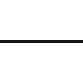
\includegraphics[valign=m, width=1cm]{figures/string2.pdf} \otimes
        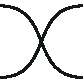
\includegraphics[valign=m, width=1cm]{figures/string1.pdf} \Bigg) \circ 
        \Bigg(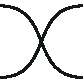
\includegraphics[valign=m, width=1cm]{figures/string1.pdf} \otimes
        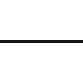
\includegraphics[valign=m, width=1cm]{figures/string2.pdf} \Bigg)$\\
        \vspace{.5cm}
        $=$\\
        \vspace{.5cm}
        $(id \otimes \gamma) \circ (\gamma \otimes id)$\\
        \vspace{.5cm}
        $=$\\
        \vspace{.5cm}
        $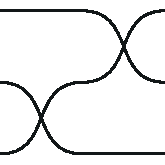
\includegraphics[valign=m, width=2cm]{figures/dia1.pdf}$\\
        
        
    \end{center}
\end{frame}


\section{Presenting finite sets and functions}
\begin{frame}
    \frametitle{Presenting finite sets and functions}
    So what can we do with $id, \gamma, \mu$ and $\eta$?
    \par
    Say we have function $f : [5] \to [5]$ (where $[n] = \{0\hdots n-1\}$):
    \begin{align*}
        f(0) &= 1\\
        f(1) &= 0\\
        f(2) &= 4\\
        f(3) &= 3\\
        f(4) &= 1
    \end{align*}

\end{frame}

\begin{frame}
    \frametitle{Presenting finite sets and functions}
    So what can we do with $id, \gamma, \mu$ and $\eta$?
    \par
    We can express this function as a string diagram:
    \begin{center}
        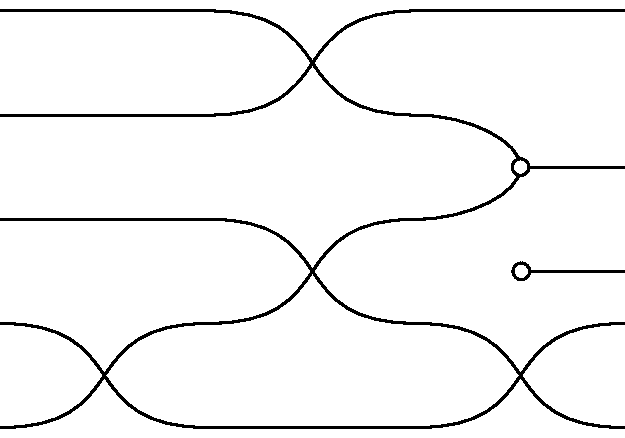
\includegraphics[height=4.5cm,keepaspectratio]{figures/dia2.pdf}
    \end{center}

\end{frame}


\begin{frame}
    \frametitle{Presenting finite sets and functions}
    So what can we do with $id, \gamma, \mu$ and $\eta$?
    \par
    Or alternatively:
    \vspace*{\fill}
    \begin{center}
        $(id \otimes id \otimes id \otimes \gamma)\ \circ$\\
        $(\gamma \otimes \gamma \otimes id)\ \circ$\\
        $(id \otimes \mu \otimes \eta \otimes \gamma)$
    \end{center}
    \vspace*{\fill}
\end{frame}

\begin{frame}
    \frametitle{String diagram equations}

    \begin{table}[]
        \centering
        \begin{tabular}{cc}
            \reflectbox{\includegraphics[valign=m, width=1.5cm]{figures/equations/e11.pdf}} = 
            \reflectbox{\includegraphics[valign=m, width=1.5cm]{figures/equations/e12.pdf}} &
            \reflectbox{\includegraphics[valign=m, width=1.5cm]{figures/equations/e21.pdf}} = 
            \reflectbox{\includegraphics[valign=m, width=1.5cm]{figures/equations/e22.pdf}} \\
            \includegraphics[valign=m, width=1.5cm]{figures/equations/e101.pdf} = 
            \includegraphics[valign=m, width=1.5cm]{figures/equations/e102.pdf} &
            \reflectbox{\rotatebox[origin=c]{180}{\includegraphics[valign=m, width=1.5cm]{figures/equations/e101.pdf}}} = 
            \reflectbox{\rotatebox[origin=c]{180}{\includegraphics[valign=m, width=1.5cm]{figures/equations/e102.pdf}}} \\

            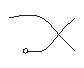
\includegraphics[valign=m, width=1.5cm]{figures/equations/e92.pdf} = 
            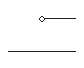
\includegraphics[valign=m, width=1.5cm]{figures/equations/e91.pdf} &
            \reflectbox{\rotatebox[origin=c]{180}{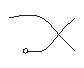
\includegraphics[valign=m, width=1.5cm]{figures/equations/e92.pdf}}} = 
            \reflectbox{\rotatebox[origin=c]{180}{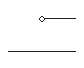
\includegraphics[valign=m, width=1.5cm]{figures/equations/e91.pdf}}} \\
            
            \includegraphics[valign=m, width=1.5cm]{figures/equations/e31.pdf} = 
            \reflectbox{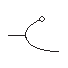
\includegraphics[valign=m, width=1.5cm]{figures/equations/e5.pdf}} &
            \includegraphics[valign=m, width=1.5cm]{figures/equations/e31.pdf} = 
            \rotatebox[origin=c]{180}{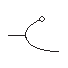
\includegraphics[valign=m, width=1.5cm]{figures/equations/e5.pdf}}\\

            \includegraphics[valign=m, width=1.5cm]{figures/equations/e41.pdf} = 
            \includegraphics[valign=m, width=1.5cm]{figures/equations/e42.pdf} &
            \includegraphics[valign=m, width=1.5cm]{figures/equations/e71.pdf} = 
            \includegraphics[valign=m, width=1.5cm]{figures/equations/e72.pdf}
            % \includegraphics[valign=m, width=1cm]{figures/equations/e31.pdf} = 
            % \includegraphics[valign=m, width=1cm]{figures/equations/e32.pdf} &

        \end{tabular}
    \end{table}
\end{frame}

\begin{frame}
    \frametitle{Presenting finite sets and functions}
    More formally, the category of functions on finite sets $\bf{F}$, is \textit{presented by} the string diagram rewriting system.
    \par
    Our category $\bf{F}$ has natural numbers $n,m \in \mathbb{N}$ as objects and arrows $f_{\bf{F}} : n \to m$ functions $f : [n] \to [m]$.
    \par
    We can turn $\bf{F}$ into a symmetric monoidal category, by defining a bifunctor $\otimes : \bf{F} \times \bf{F} \to \bf{F}$ and pick an identity object $\bf{I}$.
    \par
    We can chose $\mathrm{0}$ as our identity object (remember objects in $\bf{F}$ are natural numbers) and define $\otimes$ to be $n \otimes m = n + m$ on objects and "disjoint union" on functions, namely:
\end{frame}

\begin{frame}
    \frametitle{Presenting finite sets and functions}
    Given arrows $f_{\bf{F}} : k \to l$ and $g_{\bf{F}} : m \to n$, which are the functions $f : [k] \to [l]$ and $g : [m] \to [n]$, we define the arrow $f_{\bf{F}} \otimes g_{\bf{F}} : k+m \to l+n$ to be the function:
    \vspace{-0.3cm}
    \begin{center}
    \begin{align*}
        &f \otimes g : [k+m] \to [l+n]\\
        &f \otimes g\ (x) = \begin{cases}
            f(x) & \text{if }x < k\\
            g(x-k) +l & otherwise
        \end{cases}
    \end{align*}
    \end{center}
    Essentially stacking one function disjointly on top of the other.\par

    % We won't discuss the ``symmetric" part here, but it essentially means we have a natural isomorphism $s_{n,m} : n \otimes m \to m \otimes n$.
\end{frame}

\begin{frame}
    \frametitle{Presenting finite sets and functions}
    \vspace*{\fill}
    \begin{center}
        What do we get, if we remove $\gamma$ from our theory?\\
        \visible<2->{{\color{uolred}Linear orders and monotone maps}}\par
        What do we get, if we remove $\mu$?\\
        \visible<3->{{\color{uolred}Finite sets and injective functions}}\par
        What do we get, if we remove $\eta$?\\
        \visible<4->{{\color{uolred}Finite sets and surjective functions}}\par
        What do we get, if we remove $\mu$ and $\eta$?\\
        \visible<5->{{\color{uolred}Finite sets and bijective functions / Permutations}}
    \end{center}
    \vspace*{\fill}
\end{frame}


\section{Refresher on posets}

\begin{frame}
    \frametitle{Refresher on posets}
    A \textit{poset} is a set $S$, together with a partial order relation $\leq_S\ : S \times S$, which is \textit{reflexive}, \textit{transitive} and \textit{antisymmetric}.

    For example, for $S = \{a,b,c,d,e\}$ and $a \leq_S c ,\allowbreak a \leq_S d,\allowbreak b \leq_S d,\allowbreak c \leq_S e,\allowbreak d \leq_S e$, we can draw the following diagram, representing the poset:
    \begin{center}
    \begin{tikzpicture}
    \node (a) at (0,0) {$a$};
    \node (c) at (-1,1) {$c$};
    \node (d) at (1,1) {$d$};
    \node (e) at (0,2) {$e$};
    \node (b) at (2,0) {$b$};
    \node (f) at (2,2) {$f$};
    \draw (a) -- (c);
    \draw (a) -- (d);
    \draw (b) -- (d);
    \draw (c) -- (e);
    \draw (d) -- (e);
    \draw (d) -- (f);
    \end{tikzpicture}
    \end{center}
\end{frame}

\section{Presenting posets}

\begin{frame}
    \frametitle{Presenting posets}
    \vspace*{\fill}
    \begin{center}
    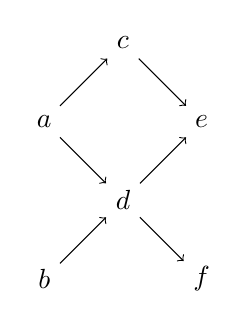
\begin{tikzpicture}
    \node (a) at (0,0) {$a$};
    \node (b) at (0,-2) {$b$};
    \node (c) at (1,1) {$c$};
    \node (d) at (1,-1) {$d$};
    \node (e) at (2,0) {$e$};
    \node (f) at (2, -2) {$f$};
    \draw[->] (a) -- (c);
    \draw[->] (a) -- (d);
    \draw[->] (b) -- (d);
    \draw[->] (c) -- (e);
    \draw[->] (d) -- (e);
    \draw[->] (d) -- (f);
    \end{tikzpicture}
    \end{center}
    \vspace*{\fill}
\end{frame}



\begin{frame}
    \frametitle{Presenting posets}
    \vspace*{\fill}
    \begin{center}
    \begin{tikzpicture}
    \node (a) at (0,0) {$\circ$};
    \node (b) at (0,-2) {$\circ$};
    \node (c) at (1,1) {$\circ$};
    \node (d) at (1,-1) {$\circ$};
    \node (e) at (2,0) {$\circ$};
    \node (f) at (2, -2) {$\circ$};
    \draw[->] (a) -- (c);
    \draw[->] (a) -- (d);
    \draw[->] (b) -- (d);
    \draw[->] (c) -- (e);
    \draw[->] (d) -- (e);
    \draw[->] (d) -- (f);
    \end{tikzpicture}
    \end{center}
    \vspace*{\fill}
\end{frame}

\begin{frame}
    \frametitle{Presenting posets}
    \vspace*{\fill}
    \begin{center}
    \begin{tikzpicture}
    \node (a) at (0,0) {$\circ$};
    \node (b) at (0,-2) {$\circ$};
    \node (c) at (1,1) {$\bullet$};
    \node (d) at (1,-1) {$\bullet$};
    \node (e) at (2,0) {$\circ$};
    \node (f) at (2, -2) {$\circ$};
    \draw[->] (a) -- (c);
    \draw[->] (a) -- (d);
    \draw[->] (b) -- (d);
    \draw[->] (c) -- (e);
    \draw[->] (d) -- (e);
    \draw[->] (d) -- (f);
    \end{tikzpicture}
    \end{center}
    \vspace*{\fill}
\end{frame}

\begin{frame}
    \frametitle{Presenting posets}
    \vspace*{\fill}
    \begin{center}
        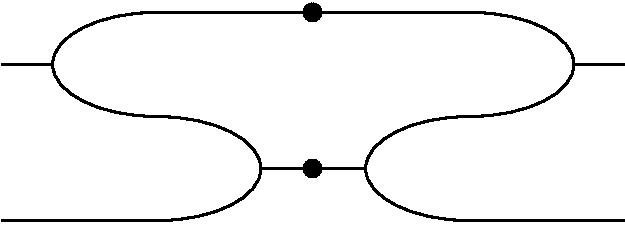
\includegraphics[height=3cm]{figures/dia3.pdf}
    \end{center}
    \vspace*{\fill}
\end{frame}

\begin{frame}
    \frametitle{Presenting posets}
    \vspace*{\fill}
    \begin{center}
        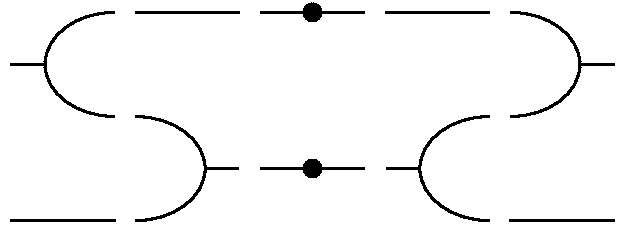
\includegraphics[height=3cm]{figures/dia4.pdf}
    \end{center}
    \vspace*{\fill}
\end{frame}

\begin{frame}
    \frametitle{Presenting posets}
    \vspace*{\fill}
    \begin{center}
        $(\delta \otimes id) \circ (id \otimes \mu) \circ (\sigma \otimes \sigma) \circ (id \otimes \delta) \circ (\mu \otimes id)$
    \end{center}
    \vspace*{\fill}
\end{frame}

\begin{frame}
    \frametitle{Presenting posets}
    We have some additional combinators in this theory:
    \vspace*{\fill}
    \begin{table}[]
        \centering
        \begin{tabular}{ccc}
            $id : 1 \to 1$ & 
            $\gamma : 2 \to 2$ & 
            \color{cyan}{$\sigma \ : 1 \to 1$}\\
            % & & \\
            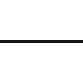
\includegraphics[valign=m, width=1cm]{figures/string2.pdf}& 
            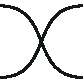
\includegraphics[valign=m, width=1cm]{figures/string1.pdf}& 
            \colorbox{cyan}{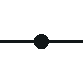
\includegraphics[valign=m, width=1cm]{figures/string5.pdf}}\\
        \end{tabular}
    \end{table}
    \begin{table}[]
        \centering
        \begin{tabular}{cccc}
            $\mu \ : 2 \to 1$ & 
            \color{cyan}{$\delta \ : 1 \to 2$} & 
            $\eta \ : 0 \to 1$&
            \color{cyan}{$\varepsilon \ : 1 \to 0$}\\
            % & & & \\
            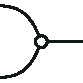
\includegraphics[valign=m, width=1cm]{figures/string4.pdf}&
            \colorbox{cyan}{\reflectbox{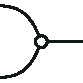
\includegraphics[valign=m, width=1cm]{figures/string4.pdf}}}&
            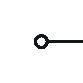
\includegraphics[valign=m, width=1cm]{figures/string3.pdf}&
            \colorbox{cyan}{\reflectbox{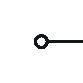
\includegraphics[valign=m, width=1cm]{figures/string3.pdf}}}\\
        \end{tabular}
    \end{table}
    \vspace*{\fill}
\end{frame}

\begin{frame}
    \frametitle{String diagram equations}

    \begin{table}[]
        \centering
        \begin{tabular}{cccc}
            \reflectbox{\includegraphics[valign=m, width=1cm]{figures/equations/e11.pdf}} = 
            \reflectbox{\includegraphics[valign=m, width=1cm]{figures/equations/e12.pdf}} &
            \reflectbox{\includegraphics[valign=m, width=1cm]{figures/equations/e21.pdf}} = 
            \reflectbox{\includegraphics[valign=m, width=1cm]{figures/equations/e22.pdf}} &
            % mirror
            & \\


            \includegraphics[valign=m, width=1cm]{figures/equations/e101.pdf} = 
            \includegraphics[valign=m, width=1cm]{figures/equations/e102.pdf} &
            \reflectbox{\rotatebox[origin=c]{180}{\includegraphics[valign=m, width=1cm]{figures/equations/e101.pdf}}} = 
            \reflectbox{\rotatebox[origin=c]{180}{\includegraphics[valign=m, width=1cm]{figures/equations/e102.pdf}}} &
            % mirror
            & \\


            \includegraphics[valign=m, width=1cm]{figures/equations/e92.pdf} = 
            \includegraphics[valign=m, width=1cm]{figures/equations/e91.pdf} &
            \reflectbox{\rotatebox[origin=c]{180}{\includegraphics[valign=m, width=1cm]{figures/equations/e92.pdf}}} = 
            \reflectbox{\rotatebox[origin=c]{180}{\includegraphics[valign=m, width=1cm]{figures/equations/e91.pdf}}} &
            % mirror
            & \\


            \includegraphics[valign=m, width=1cm]{figures/equations/e31.pdf} = 
            \reflectbox{\includegraphics[valign=m, width=1cm]{figures/equations/e5.pdf}} &
            \includegraphics[valign=m, width=1cm]{figures/equations/e31.pdf} = 
            \rotatebox[origin=c]{180}{\includegraphics[valign=m, width=1cm]{figures/equations/e5.pdf}} &
            % mirror
            & \\


            \includegraphics[valign=m, width=1cm]{figures/equations/e41.pdf} = 
            \includegraphics[valign=m, width=1cm]{figures/equations/e42.pdf} &
            \includegraphics[valign=m, width=1cm]{figures/equations/e71.pdf} = 
            \includegraphics[valign=m, width=1cm]{figures/equations/e72.pdf} &

            \includegraphics[valign=m, width=1cm]{figures/equations/empty.pdf}\\
            % \includegraphics[valign=m, width=1cm]{figures/equations/e132.pdf} \\


            \includegraphics[valign=m, width=1cm]{figures/equations/e132.pdf} \color{white}= 
            \includegraphics[valign=m, width=1cm]{figures/equations/e132.pdf} &
            \includegraphics[valign=m, width=1cm]{figures/equations/e132.pdf} \color{white}= 
            \includegraphics[valign=m, width=1cm]{figures/equations/e132.pdf} &

            \includegraphics[valign=m, width=1cm]{figures/equations/e132.pdf} \color{white}= 
            \includegraphics[valign=m, width=1cm]{figures/equations/e132.pdf} &
            \includegraphics[valign=m, width=1cm]{figures/equations/e132.pdf} \color{white}= 
            \includegraphics[valign=m, width=1cm]{figures/equations/e132.pdf} 

        \end{tabular}
    \end{table}
\end{frame}

\begin{frame}
    \frametitle{String diagram equations}

    \begin{table}[]
        \centering
        \begin{tabular}{cccc}
            \reflectbox{\includegraphics[valign=m, width=1cm]{figures/equations/e11.pdf}} = 
            \reflectbox{\includegraphics[valign=m, width=1cm]{figures/equations/e12.pdf}} &
            \reflectbox{\includegraphics[valign=m, width=1cm]{figures/equations/e21.pdf}} = 
            \reflectbox{\includegraphics[valign=m, width=1cm]{figures/equations/e22.pdf}} &
            % mirror
            \includegraphics[valign=m, width=1cm]{figures/equations/e22.pdf} = 
            \includegraphics[valign=m, width=1cm]{figures/equations/e21.pdf} &
            \includegraphics[valign=m, width=1cm]{figures/equations/e12.pdf} = 
            \includegraphics[valign=m, width=1cm]{figures/equations/e11.pdf} \\


            \includegraphics[valign=m, width=1cm]{figures/equations/e101.pdf} = 
            \includegraphics[valign=m, width=1cm]{figures/equations/e102.pdf} &
            \reflectbox{\rotatebox[origin=c]{180}{\includegraphics[valign=m, width=1cm]{figures/equations/e101.pdf}}} = 
            \reflectbox{\rotatebox[origin=c]{180}{\includegraphics[valign=m, width=1cm]{figures/equations/e102.pdf}}} &
            % mirror
            \rotatebox[origin=c]{180}{\includegraphics[valign=m, width=1cm]{figures/equations/e102.pdf}} = 
            \rotatebox[origin=c]{180}{\includegraphics[valign=m, width=1cm]{figures/equations/e101.pdf}} &
            \reflectbox{\includegraphics[valign=m, width=1cm]{figures/equations/e102.pdf}} = 
            \reflectbox{\includegraphics[valign=m, width=1cm]{figures/equations/e101.pdf}} \\


            \includegraphics[valign=m, width=1cm]{figures/equations/e92.pdf} = 
            \includegraphics[valign=m, width=1cm]{figures/equations/e91.pdf} &
            \reflectbox{\rotatebox[origin=c]{180}{\includegraphics[valign=m, width=1cm]{figures/equations/e92.pdf}}} = 
            \reflectbox{\rotatebox[origin=c]{180}{\includegraphics[valign=m, width=1cm]{figures/equations/e91.pdf}}} &
            % mirror
            \rotatebox[origin=c]{180}{\includegraphics[valign=m, width=1cm]{figures/equations/e91.pdf}} = 
            \rotatebox[origin=c]{180}{\includegraphics[valign=m, width=1cm]{figures/equations/e92.pdf}} &
            \reflectbox{\includegraphics[valign=m, width=1cm]{figures/equations/e91.pdf}} = 
            \reflectbox{\includegraphics[valign=m, width=1cm]{figures/equations/e92.pdf}} \\


            \includegraphics[valign=m, width=1cm]{figures/equations/e31.pdf} = 
            \reflectbox{\includegraphics[valign=m, width=1cm]{figures/equations/e5.pdf}} &
            \includegraphics[valign=m, width=1cm]{figures/equations/e31.pdf} = 
            \rotatebox[origin=c]{180}{\includegraphics[valign=m, width=1cm]{figures/equations/e5.pdf}} &
            % mirror
            \reflectbox{\rotatebox[origin=c]{180}{\includegraphics[valign=m, width=1cm]{figures/equations/e5.pdf}}} = 
            \includegraphics[valign=m, width=1cm]{figures/equations/e31.pdf} &
            \includegraphics[valign=m, width=1cm]{figures/equations/e5.pdf} = 
            \includegraphics[valign=m, width=1cm]{figures/equations/e31.pdf}\\


            \includegraphics[valign=m, width=1cm]{figures/equations/e41.pdf} = 
            \includegraphics[valign=m, width=1cm]{figures/equations/e42.pdf} &
            \includegraphics[valign=m, width=1cm]{figures/equations/e71.pdf} = 
            \includegraphics[valign=m, width=1cm]{figures/equations/e72.pdf} &
            \includegraphics[valign=m, width=1cm]{figures/equations/e142.pdf} = 
            \includegraphics[valign=m, width=1cm]{figures/equations/e141.pdf} &
            \includegraphics[valign=m, width=1cm]{figures/equations/e131.pdf} = 
            \includegraphics[valign=m, width=1cm]{figures/equations/e132.pdf} \\


            \includegraphics[valign=m, width=1cm]{figures/equations/e31.pdf} = 
            \includegraphics[valign=m, width=1cm]{figures/equations/e32.pdf} &
            \includegraphics[valign=m, width=1cm]{figures/equations/e111.pdf} = 
            \rotatebox[origin=c]{180}{\includegraphics[valign=m, width=1cm]{figures/equations/e111.pdf}} &

            \rotatebox[origin=c]{180}{\reflectbox{\includegraphics[valign=m, width=1cm]{figures/equations/e111.pdf}}} = 
            \reflectbox{\includegraphics[valign=m, width=1cm]{figures/equations/e111.pdf}} &

            \includegraphics[valign=m, width=1cm]{figures/equations/e121.pdf} = 
            \includegraphics[valign=m, width=1cm]{figures/equations/e122.pdf}

        \end{tabular}
    \end{table}
\end{frame}

\section{Presenting posets and monotone functions?}

\begin{frame}
    \frametitle{Presenting posets and monotone functions?}
    \vspace*{\fill}
    \begin{center}
    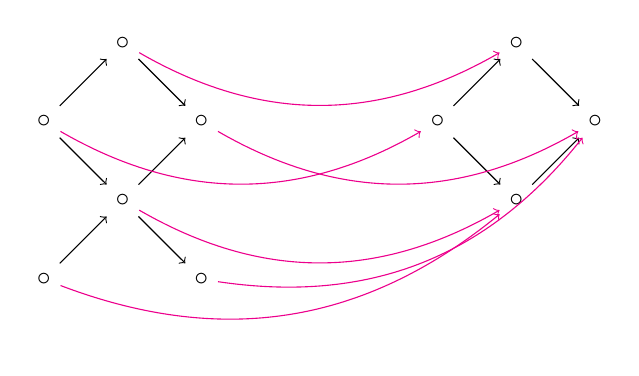
\begin{tikzpicture}
    \node (a) at (0,0) {$\circ$};
    \node (b) at (0,-2) {$\circ$};
    \node (c) at (1,1) {$\circ$};
    \node (d) at (1,-1) {$\circ$};
    \node (e) at (2,0) {$\circ$};
    \node (f) at (2, -2) {$\circ$};

    \node (aa) at (5,0) {$\circ$};
    \node (bb) at (6,1) {$\circ$};
    \node (cc) at (6,-1) {$\circ$};
    \node (dd) at (7,0) {$\circ$};
    \draw[->] (a) -- (c);
    \draw[->] (a) -- (d);
    \draw[->] (b) -- (d);
    \draw[->] (c) -- (e);
    \draw[->] (d) -- (e);
    \draw[->] (d) -- (f);

    \draw[->] (aa) -- (bb);
    \draw[->] (aa) -- (cc);
    \draw[->] (bb) -- (dd);
    \draw[->] (cc) -- (dd);

    \visible<2->{
    \draw[->, magenta] (a) to [bend right] (aa);
    \draw[->, magenta] (b) to [bend right] (cc);
    \draw[->, magenta] (c) to [bend right] (bb);
    \draw[->, magenta] (d) to [bend right] (cc);
    \draw[->, magenta] (e) to [bend right] (dd);
    \draw[->, magenta] (f) to [bend right] (dd);}
    \end{tikzpicture}
    \end{center}
    \vspace*{\fill}
\end{frame}


\begin{frame}
    \frametitle{Presenting posets and monotone functions?}
    \vspace*{\fill}
    \begin{center}
    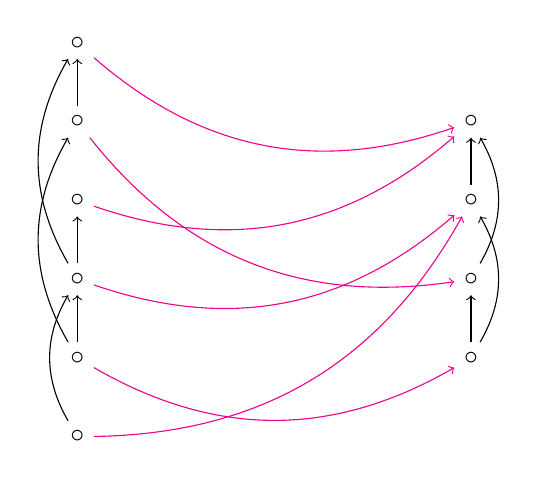
\begin{tikzpicture}
    \node (a) at (0,1) {$\circ$};
    \node (b) at (0,0) {$\circ$};
    \node (c) at (0,4) {$\circ$};
    \node (d) at (0,2) {$\circ$};
    \node (e) at (0,5) {$\circ$};
    \node (f) at (0,3) {$\circ$};

    \node (aa) at (5,1) {$\circ$};
    \node (bb) at (5,2) {$\circ$};
    \node (cc) at (5,3) {$\circ$};
    \node (dd) at (5,4) {$\circ$};
    \draw[->] (a) to [bend left] (c);
    \draw[->] (a) -- (d);
    \draw[->] (b) to [bend left] (d);
    \draw[->] (c) -- (e);
    \draw[->] (d) to [bend left] (e);
    \draw[->] (d) -- (f);

    \draw[->] (aa) -- (bb);
    \draw[->] (aa) to [bend right] (cc);
    \draw[->] (bb) to [bend right] (dd);
    \draw[->] (cc) -- (dd);

    \visible<2->{
    \draw[->, magenta] (a) to [bend right] (aa);
    \draw[->, magenta] (b) to [bend right] (cc);
    \draw[->, magenta] (c) to [bend right] (bb);
    \draw[->, magenta] (d) to [bend right] (cc);
    \draw[->, magenta] (e) to [bend right] (dd);
    \draw[->, magenta] (f) to [bend right] (dd);}
    \end{tikzpicture}
    \end{center}
    \vspace*{\fill}
\end{frame}

\begin{frame}
    \frametitle{Who's stuff I \st{stole} borrowed}
    Drawing string diagrams is quite tedious!\par
    I therefore borrowed some excellent ones from Pawel Sobocinski's \href{http://www.cs.le.ac.uk/events/mgs2017/courses/graphical-linear-algebra.html}{MGS 2017 lecture notes} (also, checkout his blog on \href{https://graphicallinearalgebra.net}{Graphical Linear Algebra!}) \\(p. 3-4)\par
    I also used some string diagrams from S. Mimram's paper \href{https://arxiv.org/pdf/1505.07161.pdf}{Presenting Finite Posets}, on which this presentation was based \\(p. 11,27)
\end{frame}


\lastframe%
\end{document}
